\documentclass{standalone}
\usepackage{tikz}
\usetikzlibrary{patterns, positioning}


\begin{document}
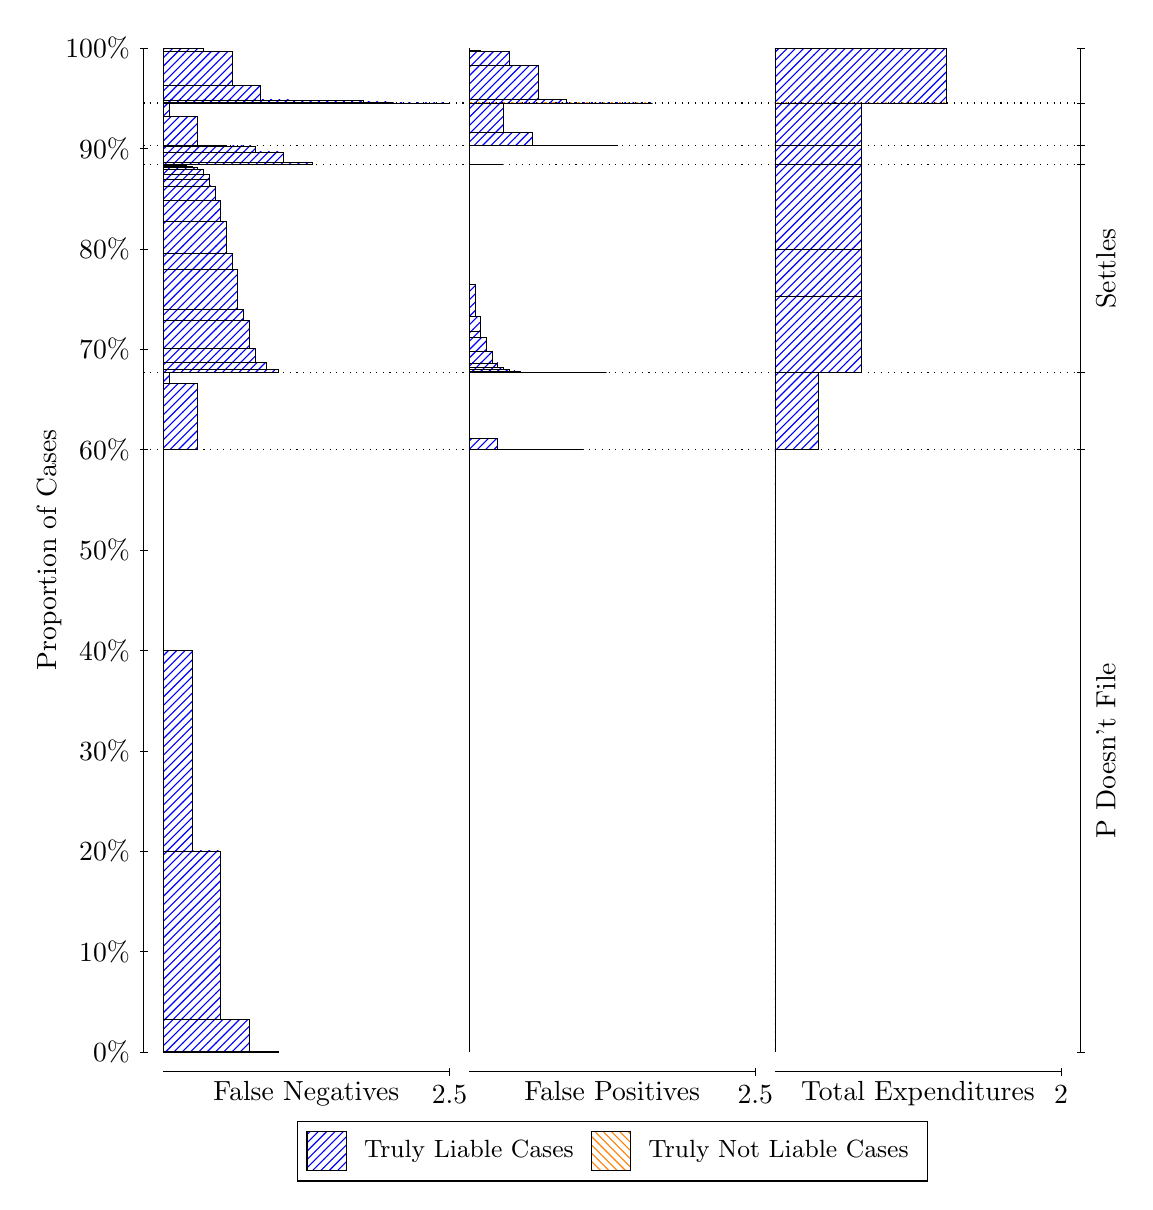
\begin{tikzpicture}
\draw[black, very thin] (1.5,1.75) -- (1.5,14.5);
\node[rotate=90, text=black, anchor=center] at (0.3, 8.125) {Proportion of Cases};
\draw[black, very thin] (1.45,1.75) -- (1.55,1.75);
\node[text=black, anchor=east] at (1.45, 1.75) {0\%};
\draw[black, very thin] (1.45,3.025) -- (1.55,3.025);
\node[text=black, anchor=east] at (1.45, 3.025) {10\%};
\draw[black, very thin] (1.45,4.3) -- (1.55,4.3);
\node[text=black, anchor=east] at (1.45, 4.3) {20\%};
\draw[black, very thin] (1.45,5.575) -- (1.55,5.575);
\node[text=black, anchor=east] at (1.45, 5.575) {30\%};
\draw[black, very thin] (1.45,6.85) -- (1.55,6.85);
\node[text=black, anchor=east] at (1.45, 6.85) {40\%};
\draw[black, very thin] (1.45,8.125) -- (1.55,8.125);
\node[text=black, anchor=east] at (1.45, 8.125) {50\%};
\draw[black, very thin] (1.45,9.4) -- (1.55,9.4);
\node[text=black, anchor=east] at (1.45, 9.4) {60\%};
\draw[black, very thin] (1.45,10.675) -- (1.55,10.675);
\node[text=black, anchor=east] at (1.45, 10.675) {70\%};
\draw[black, very thin] (1.45,11.95) -- (1.55,11.95);
\node[text=black, anchor=east] at (1.45, 11.95) {80\%};
\draw[black, very thin] (1.45,13.225) -- (1.55,13.225);
\node[text=black, anchor=east] at (1.45, 13.225) {90\%};
\draw[black, very thin] (1.45,14.5) -- (1.55,14.5);
\node[text=black, anchor=east] at (1.45, 14.5) {100\%};

\draw[black, very thin] (13.4,1.75) -- (13.4,14.5);
\draw[black, very thin] (13.35,1.75) -- (13.45,1.75);
\node[anchor=west] at (13.35, 1.75) {};
\draw[black, very thin] (13.35,9.4013) -- (13.45,9.4013);
\node[anchor=west] at (13.35, 9.4013) {};
\draw[black, very thin] (13.35,10.379) -- (13.45,10.379);
\node[anchor=west] at (13.35, 10.379) {};
\draw[black, very thin] (13.35,13.02) -- (13.45,13.02);
\node[anchor=west] at (13.35, 13.02) {};
\draw[black, very thin] (13.35,13.26) -- (13.45,13.26);
\node[anchor=west] at (13.35, 13.26) {};
\draw[black, very thin] (13.35,13.802) -- (13.45,13.802);
\node[anchor=west] at (13.35, 13.802) {};
\draw[black, very thin] (13.35,14.5) -- (13.45,14.5);
\node[anchor=west] at (13.35, 14.5) {};

\draw[black, very thin, pattern color=blue, pattern=north east lines] (1.75,1.75) rectangle (3.2033,1.7541);
\draw[black, very thin, pattern color=blue, pattern=north east lines] (1.75,1.7541) rectangle (2.84,2.1592);
\draw[black, very thin, pattern color=blue, pattern=north east lines] (1.75,2.1592) rectangle (2.4767,4.3047);
\draw[black, very thin, pattern color=blue, pattern=north east lines] (1.75,4.3047) rectangle (2.1133,6.8513);
\draw[black, very thin, pattern color=orange, pattern=north west lines] (1.75,6.8513) rectangle (1.75,6.8513);
\draw[black, very thin, pattern color=blue, pattern=north east lines] (1.75,6.8513) rectangle (1.75,9.4013);
\draw[black, very thin, pattern color=blue, pattern=north east lines] (1.75,9.4013) rectangle (2.186,10.241);
\draw[black, very thin, pattern color=blue, pattern=north east lines] (1.75,10.241) rectangle (1.8227,10.378);
\draw[black, very thin, pattern color=orange, pattern=north west lines] (1.75,10.378) rectangle (1.75,10.378);
\draw[black, very thin, pattern color=blue, pattern=north east lines] (1.75,10.378) rectangle (1.75,10.379);
\draw[black, very thin, pattern color=blue, pattern=north east lines] (1.75,10.379) rectangle (3.2033,10.421);
\draw[black, very thin, pattern color=blue, pattern=north east lines] (1.75,10.421) rectangle (3.058,10.508);
\draw[black, very thin, pattern color=blue, pattern=north east lines] (1.75,10.508) rectangle (2.9127,10.689);
\draw[black, very thin, pattern color=blue, pattern=north east lines] (1.75,10.689) rectangle (2.84,11.046);
\draw[black, very thin, pattern color=blue, pattern=north east lines] (1.75,11.046) rectangle (2.7673,11.178);
\draw[black, very thin, pattern color=blue, pattern=north east lines] (1.75,11.178) rectangle (2.6947,11.688);
\draw[black, very thin, pattern color=blue, pattern=north east lines] (1.75,11.688) rectangle (2.622,11.897);
\draw[black, very thin, pattern color=blue, pattern=north east lines] (1.75,11.897) rectangle (2.5493,12.303);
\draw[black, very thin, pattern color=blue, pattern=north east lines] (1.75,12.303) rectangle (2.4767,12.569);
\draw[black, very thin, pattern color=blue, pattern=north east lines] (1.75,12.569) rectangle (2.404,12.748);
\draw[black, very thin, pattern color=blue, pattern=north east lines] (1.75,12.748) rectangle (2.3313,12.829);
\draw[black, very thin, pattern color=blue, pattern=north east lines] (1.75,12.829) rectangle (2.3313,12.896);
\draw[black, very thin, pattern color=blue, pattern=north east lines] (1.75,12.896) rectangle (2.2587,12.957);
\draw[black, very thin, pattern color=blue, pattern=north east lines] (1.75,12.957) rectangle (2.186,12.981);
\draw[black, very thin, pattern color=blue, pattern=north east lines] (1.75,12.981) rectangle (2.1133,12.998);
\draw[black, very thin, pattern color=blue, pattern=north east lines] (1.75,12.998) rectangle (2.0407,13.006);
\draw[black, very thin, pattern color=blue, pattern=north east lines] (1.75,13.006) rectangle (1.968,13.006);
\draw[black, very thin, pattern color=blue, pattern=north east lines] (1.75,13.006) rectangle (1.968,13.019);
\draw[black, very thin, pattern color=blue, pattern=north east lines] (1.75,13.019) rectangle (1.8953,13.02);
\draw[black, very thin, pattern color=blue, pattern=north east lines] (1.75,13.02) rectangle (1.8227,13.02);
\draw[black, very thin, pattern color=orange, pattern=north west lines] (1.75,13.02) rectangle (1.75,13.02);
\draw[black, very thin, pattern color=blue, pattern=north east lines] (1.75,13.02) rectangle (1.75,13.02);
\draw[black, very thin, pattern color=blue, pattern=north east lines] (1.75,13.02) rectangle (3.6393,13.052);
\draw[black, very thin, pattern color=blue, pattern=north east lines] (1.75,13.052) rectangle (3.276,13.181);
\draw[black, very thin, pattern color=blue, pattern=north east lines] (1.75,13.181) rectangle (2.9127,13.257);
\draw[black, very thin, pattern color=blue, pattern=north east lines] (1.75,13.257) rectangle (2.5493,13.26);
\draw[black, very thin, pattern color=blue, pattern=north east lines] (1.75,13.26) rectangle (2.186,13.26);
\draw[black, very thin, pattern color=orange, pattern=north west lines] (1.75,13.26) rectangle (1.75,13.26);
\draw[black, very thin, pattern color=blue, pattern=north east lines] (1.75,13.26) rectangle (2.186,13.632);
\draw[black, very thin, pattern color=blue, pattern=north east lines] (1.75,13.632) rectangle (1.8227,13.797);
\draw[black, very thin, pattern color=orange, pattern=north west lines] (1.75,13.797) rectangle (1.75,13.797);
\draw[black, very thin, pattern color=blue, pattern=north east lines] (1.75,13.797) rectangle (1.75,13.802);
\draw[black, very thin, pattern color=blue, pattern=north east lines] (1.75,13.802) rectangle (5.3833,13.802);
\draw[black, very thin, pattern color=blue, pattern=north east lines] (1.75,13.802) rectangle (5.02,13.802);
\draw[black, very thin, pattern color=blue, pattern=north east lines] (1.75,13.802) rectangle (4.6567,13.815);
\draw[black, very thin, pattern color=blue, pattern=north east lines] (1.75,13.815) rectangle (4.2933,13.834);
\draw[black, very thin, pattern color=blue, pattern=north east lines] (1.75,13.834) rectangle (3.93,13.835);
\draw[black, very thin, pattern color=blue, pattern=north east lines] (1.75,13.835) rectangle (3.712,13.835);
\draw[black, very thin, pattern color=blue, pattern=north east lines] (1.75,13.835) rectangle (3.5667,13.835);
\draw[black, very thin, pattern color=blue, pattern=north east lines] (1.75,13.835) rectangle (3.3487,13.841);
\draw[black, very thin, pattern color=blue, pattern=north east lines] (1.75,13.841) rectangle (3.2033,13.841);
\draw[black, very thin, pattern color=blue, pattern=north east lines] (1.75,13.841) rectangle (2.9853,14.023);
\draw[black, very thin, pattern color=blue, pattern=north east lines] (1.75,14.023) rectangle (2.622,14.455);
\draw[black, very thin, pattern color=blue, pattern=north east lines] (1.75,14.455) rectangle (2.2587,14.5);
\draw[black, very thin, pattern color=blue, pattern=north east lines] (1.75,14.5) rectangle (1.8953,14.5);
\draw[black, very thin, pattern color=orange, pattern=north west lines] (1.75,14.5) rectangle (1.75,14.5);
\draw[black, very thin, pattern color=blue, pattern=north east lines] (1.75,14.5) rectangle (1.75,14.5);
\draw[black, very thin, pattern color=orange, pattern=north west lines] (5.6333,1.75) rectangle (5.6333,1.75);
\draw[black, very thin, pattern color=blue, pattern=north east lines] (5.6333,1.75) rectangle (5.6333,9.4013);
\draw[black, very thin, pattern color=orange, pattern=north west lines] (5.6333,9.4013) rectangle (7.0867,9.4013);
\draw[black, very thin, pattern color=blue, pattern=north east lines] (5.6333,9.4013) rectangle (7.0867,9.4013);
\draw[black, very thin, pattern color=blue, pattern=north east lines] (5.6333,9.4013) rectangle (6.7233,9.4013);
\draw[black, very thin, pattern color=blue, pattern=north east lines] (5.6333,9.4013) rectangle (6.36,9.4015);
\draw[black, very thin, pattern color=blue, pattern=north east lines] (5.6333,9.4015) rectangle (5.9967,9.5389);
\draw[black, very thin, pattern color=blue, pattern=north east lines] (5.6333,9.5389) rectangle (5.6333,10.379);
\draw[black, very thin, pattern color=orange, pattern=north west lines] (5.6333,10.379) rectangle (7.3773,10.379);
\draw[black, very thin, pattern color=blue, pattern=north east lines] (5.6333,10.379) rectangle (7.3773,10.379);
\draw[black, very thin, pattern color=orange, pattern=north west lines] (5.6333,10.379) rectangle (7.232,10.379);
\draw[black, very thin, pattern color=blue, pattern=north east lines] (5.6333,10.379) rectangle (7.232,10.379);
\draw[black, very thin, pattern color=orange, pattern=north west lines] (5.6333,10.379) rectangle (7.0867,10.379);
\draw[black, very thin, pattern color=blue, pattern=north east lines] (5.6333,10.379) rectangle (7.0867,10.379);
\draw[black, very thin, pattern color=blue, pattern=north east lines] (5.6333,10.379) rectangle (7.014,10.379);
\draw[black, very thin, pattern color=orange, pattern=north west lines] (5.6333,10.379) rectangle (6.9413,10.379);
\draw[black, very thin, pattern color=blue, pattern=north east lines] (5.6333,10.379) rectangle (6.9413,10.379);
\draw[black, very thin, pattern color=blue, pattern=north east lines] (5.6333,10.379) rectangle (6.8687,10.379);
\draw[black, very thin, pattern color=orange, pattern=north west lines] (5.6333,10.379) rectangle (6.796,10.379);
\draw[black, very thin, pattern color=blue, pattern=north east lines] (5.6333,10.379) rectangle (6.796,10.379);
\draw[black, very thin, pattern color=blue, pattern=north east lines] (5.6333,10.379) rectangle (6.7233,10.379);
\draw[black, very thin, pattern color=orange, pattern=north west lines] (5.6333,10.379) rectangle (6.6507,10.379);
\draw[black, very thin, pattern color=blue, pattern=north east lines] (5.6333,10.379) rectangle (6.6507,10.379);
\draw[black, very thin, pattern color=blue, pattern=north east lines] (5.6333,10.379) rectangle (6.578,10.379);
\draw[black, very thin, pattern color=blue, pattern=north east lines] (5.6333,10.379) rectangle (6.5053,10.379);
\draw[black, very thin, pattern color=orange, pattern=north west lines] (5.6333,10.379) rectangle (6.5053,10.379);
\draw[black, very thin, pattern color=blue, pattern=north east lines] (5.6333,10.379) rectangle (6.5053,10.379);
\draw[black, very thin, pattern color=blue, pattern=north east lines] (5.6333,10.379) rectangle (6.4327,10.379);
\draw[black, very thin, pattern color=blue, pattern=north east lines] (5.6333,10.379) rectangle (6.36,10.38);
\draw[black, very thin, pattern color=blue, pattern=north east lines] (5.6333,10.38) rectangle (6.2873,10.393);
\draw[black, very thin, pattern color=blue, pattern=north east lines] (5.6333,10.393) rectangle (6.2147,10.401);
\draw[black, very thin, pattern color=blue, pattern=north east lines] (5.6333,10.401) rectangle (6.142,10.418);
\draw[black, very thin, pattern color=blue, pattern=north east lines] (5.6333,10.418) rectangle (6.142,10.418);
\draw[black, very thin, pattern color=blue, pattern=north east lines] (5.6333,10.418) rectangle (6.0693,10.442);
\draw[black, very thin, pattern color=blue, pattern=north east lines] (5.6333,10.442) rectangle (5.9967,10.502);
\draw[black, very thin, pattern color=blue, pattern=north east lines] (5.6333,10.502) rectangle (5.924,10.651);
\draw[black, very thin, pattern color=blue, pattern=north east lines] (5.6333,10.651) rectangle (5.8513,10.829);
\draw[black, very thin, pattern color=blue, pattern=north east lines] (5.6333,10.829) rectangle (5.7787,10.905);
\draw[black, very thin, pattern color=blue, pattern=north east lines] (5.6333,10.905) rectangle (5.7787,11.096);
\draw[black, very thin, pattern color=blue, pattern=north east lines] (5.6333,11.096) rectangle (5.706,11.502);
\draw[black, very thin, pattern color=blue, pattern=north east lines] (5.6333,11.502) rectangle (5.6333,13.02);
\draw[black, very thin, pattern color=orange, pattern=north west lines] (5.6333,13.02) rectangle (6.0693,13.02);
\draw[black, very thin, pattern color=blue, pattern=north east lines] (5.6333,13.02) rectangle (6.0693,13.02);
\draw[black, very thin, pattern color=blue, pattern=north east lines] (5.6333,13.02) rectangle (5.706,13.023);
\draw[black, very thin, pattern color=blue, pattern=north east lines] (5.6333,13.023) rectangle (5.6333,13.26);
\draw[black, very thin, pattern color=orange, pattern=north west lines] (5.6333,13.26) rectangle (7.5227,13.26);
\draw[black, very thin, pattern color=blue, pattern=north east lines] (5.6333,13.26) rectangle (7.5227,13.26);
\draw[black, very thin, pattern color=blue, pattern=north east lines] (5.6333,13.26) rectangle (7.1593,13.26);
\draw[black, very thin, pattern color=blue, pattern=north east lines] (5.6333,13.26) rectangle (6.796,13.265);
\draw[black, very thin, pattern color=blue, pattern=north east lines] (5.6333,13.265) rectangle (6.4327,13.43);
\draw[black, very thin, pattern color=blue, pattern=north east lines] (5.6333,13.43) rectangle (6.0693,13.802);
\draw[black, very thin, pattern color=orange, pattern=north west lines] (5.6333,13.802) rectangle (7.9587,13.802);
\draw[black, very thin, pattern color=blue, pattern=north east lines] (5.6333,13.802) rectangle (7.9587,13.802);
\draw[black, very thin, pattern color=orange, pattern=north west lines] (5.6333,13.802) rectangle (7.5953,13.802);
\draw[black, very thin, pattern color=blue, pattern=north east lines] (5.6333,13.802) rectangle (7.5953,13.802);
\draw[black, very thin, pattern color=orange, pattern=north west lines] (5.6333,13.802) rectangle (7.232,13.802);
\draw[black, very thin, pattern color=blue, pattern=north east lines] (5.6333,13.802) rectangle (7.232,13.802);
\draw[black, very thin, pattern color=blue, pattern=north east lines] (5.6333,13.802) rectangle (6.8687,13.847);
\draw[black, very thin, pattern color=orange, pattern=north west lines] (5.6333,13.847) rectangle (6.8687,13.847);
\draw[black, very thin, pattern color=blue, pattern=north east lines] (5.6333,13.847) rectangle (6.8687,13.847);
\draw[black, very thin, pattern color=blue, pattern=north east lines] (5.6333,13.847) rectangle (6.5053,14.279);
\draw[black, very thin, pattern color=blue, pattern=north east lines] (5.6333,14.279) rectangle (6.5053,14.279);
\draw[black, very thin, pattern color=blue, pattern=north east lines] (5.6333,14.279) rectangle (6.142,14.458);
\draw[black, very thin, pattern color=blue, pattern=north east lines] (5.6333,14.458) rectangle (6.142,14.46);
\draw[black, very thin, pattern color=orange, pattern=north west lines] (5.6333,14.46) rectangle (5.924,14.46);
\draw[black, very thin, pattern color=blue, pattern=north east lines] (5.6333,14.46) rectangle (5.924,14.46);
\draw[black, very thin, pattern color=blue, pattern=north east lines] (5.6333,14.46) rectangle (5.7787,14.466);
\draw[black, very thin, pattern color=blue, pattern=north east lines] (5.6333,14.466) rectangle (5.7787,14.467);
\draw[black, very thin, pattern color=orange, pattern=north west lines] (5.6333,14.467) rectangle (5.6333,14.467);
\draw[black, very thin, pattern color=blue, pattern=north east lines] (5.6333,14.467) rectangle (5.6333,14.5);
\draw[black, very thin, pattern color=orange, pattern=north west lines] (9.5167,1.75) rectangle (9.5167,1.75);
\draw[black, very thin, pattern color=blue, pattern=north east lines] (9.5167,1.75) rectangle (9.5167,9.4013);
\draw[black, very thin, pattern color=orange, pattern=north west lines] (9.5167,9.4013) rectangle (10.062,9.4013);
\draw[black, very thin, pattern color=blue, pattern=north east lines] (9.5167,9.4013) rectangle (10.062,10.379);
\draw[black, very thin, pattern color=orange, pattern=north west lines] (9.5167,10.379) rectangle (10.607,10.379);
\draw[black, very thin, pattern color=blue, pattern=north east lines] (9.5167,10.379) rectangle (10.607,11.353);
\draw[black, very thin, pattern color=orange, pattern=north west lines] (9.5167,11.353) rectangle (10.607,11.353);
\draw[black, very thin, pattern color=blue, pattern=north east lines] (9.5167,11.353) rectangle (10.607,11.944);
\draw[black, very thin, pattern color=orange, pattern=north west lines] (9.5167,11.944) rectangle (10.607,11.944);
\draw[black, very thin, pattern color=blue, pattern=north east lines] (9.5167,11.944) rectangle (10.607,13.02);
\draw[black, very thin, pattern color=orange, pattern=north west lines] (9.5167,13.02) rectangle (10.607,13.02);
\draw[black, very thin, pattern color=blue, pattern=north east lines] (9.5167,13.02) rectangle (10.607,13.26);
\draw[black, very thin, pattern color=orange, pattern=north west lines] (9.5167,13.26) rectangle (10.607,13.26);
\draw[black, very thin, pattern color=blue, pattern=north east lines] (9.5167,13.26) rectangle (10.607,13.802);
\draw[black, very thin, pattern color=orange, pattern=north west lines] (9.5167,13.802) rectangle (11.697,13.802);
\draw[black, very thin, pattern color=blue, pattern=north east lines] (9.5167,13.802) rectangle (11.697,14.497);
\draw[black, very thin, pattern color=orange, pattern=north west lines] (9.5167,14.497) rectangle (11.697,14.497);
\draw[black, very thin, pattern color=blue, pattern=north east lines] (9.5167,14.497) rectangle (11.697,14.5);
\draw[black, dotted] (1.5,9.4013) -- (13.4,9.4013);
\draw[black, dotted] (1.5,10.379) -- (13.4,10.379);
\draw[black, dotted] (1.5,13.02) -- (13.4,13.02);
\draw[black, dotted] (1.5,13.26) -- (13.4,13.26);
\draw[black, dotted] (1.5,13.802) -- (13.4,13.802);
\draw[black, very thin] (1.75,1.5) -- (5.3833,1.5);
\node[text=black, anchor=north] at (3.5667, 1.5) {False Negatives};
\draw[black, very thin] (5.3833,1.45) -- (5.3833,1.55);
\node[text=black, anchor=north] at (5.3833, 1.45) {2.5};

\draw[black, very thin] (5.6333,1.5) -- (9.2667,1.5);
\node[text=black, anchor=north] at (7.45, 1.5) {False Positives};
\draw[black, very thin] (9.2667,1.45) -- (9.2667,1.55);
\node[text=black, anchor=north] at (9.2667, 1.45) {2.5};

\draw[black, very thin] (9.5167,1.5) -- (13.15,1.5);
\node[text=black, anchor=north] at (11.333, 1.5) {Total Expenditures};
\draw[black, very thin] (13.15,1.45) -- (13.15,1.55);
\node[text=black, anchor=north] at (13.15, 1.45) {2};

\node[text=black, centered, rotate=90] at (13.72, 5.5756) {P Doesn't File};

\node[text=black, centered, rotate=90] at (13.72, 11.699) {Settles};




\draw (7.449999999999999,1.5) node[draw=none] (baseCoordinate) {};
\begin{scope}[align=center]
        \matrix[scale=0.5, draw=black, below=0.5cm of baseCoordinate, nodes={draw}, column sep=0.1cm]{
            \node[rectangle, draw, minimum width=0.5cm, minimum height=0.5cm, pattern color=blue, pattern=north east lines] {}; &
            \node[draw=none, font=\small, text=black] (B) {Truly Liable Cases}; &
            \node[rectangle, draw, minimum width=0.5cm, minimum height=0.5cm, pattern color=orange, pattern=north west lines] {}; &
            \node[draw=none, font=\small, text=black] (B) {Truly Not Liable Cases}; \\
            };
\end{scope}

\end{tikzpicture}
\end{document}